\documentclass[10pt]{article}
\usepackage{amsmath,amssymb}
\setlength{\oddsidemargin}{0in}
\setlength{\evensidemargin}{0in}
\setlength{\textheight}{9in}
\setlength{\textwidth}{6.5in}
\setlength{\topmargin}{-0.5in}
\usepackage{enumitem}
\usepackage{graphicx}
\usepackage{float}
\DeclareMathOperator*{\argmax}{arg\,max}
\DeclareMathOperator*{\argmin}{arg\,min}
\title{\bf Math 170S: Homework 3}
\date{10/27/2023}
\author{\bf Owen Jones}

\begin{document}
\maketitle
\begin{enumerate}[label=\textbf{Problem \arabic*.}]
\item Want to find $a(X),b(X)$ with $C(X)=(a(X),b(X))$ s.t $P(\mu\in C(X))=0.99$. 
$\overline{x}=\frac{1}{n}\sum_{i=1}^{n}x_i=14.01429$.
Let $z_{\frac{\alpha}{2}}=2.57583$ for $\alpha=0.01$.
$a(X)=\overline{x}-z_{\frac{\alpha}{2}}\frac{\sigma}{\sqrt{n}}=11.26061$, 
$b(X)=\overline{x}+z_{\frac{\alpha}{2}}\frac{\sigma}{\sqrt{n}}=16.76796$.
Thus, $C(X)=(11.26061,16.76796)$
\item Want to find $a(X),b(X)$ with $C(X)=(a(X),b(X))$ s.t $P(\mu\in C(X))=0.95$. 
$\overline{x}=\frac{1}{n}\sum_{i=1}^{n}x_i=89.5$.
Let $t_{\frac{\alpha}{2}}^{(n-1)}=2.26216$ for $n=10$ and $\alpha=0.05$. $s_x=\sqrt{\frac{1}{n-1}\sum_{i=1}^{n}{(x_i-\overline{x})}^2}=16.58145$. 
$a(X)=\overline{x}-t_{\frac{\alpha}{2}}^{(n-1)}\frac{s_x}{\sqrt{n}}=77.63835$
$b(X)=\overline{x}+t_{\frac{\alpha}{2}}^{(n-1)}\frac{\sigma}{\sqrt{n}}=101.36165$.
Thus, $C(X)=(77.63835,101.36165)$.
\item \begin{itemize}
    \item [1.] $\pi(\lambda|x)\propto\pi(x|\lambda)\pi(\lambda)$. 
    Let $\pi(\lambda)=\Gamma(a,b)=\frac{b^a \lambda^{a-1}e^{-b\lambda}}{\Gamma(a)}$. 
    Let $\displaystyle\pi(x|\lambda)=\prod_{i=1}^{n} \lambda e^{-x_i\lambda}$.
    Thus, $\pi(\lambda|x)\propto \frac{b^a\lambda^{a+n-1}e^{-\lambda(b+\sum_{i=1}^{n}x_i)}}{\Gamma(a)}\Rightarrow\pi(\lambda|x)=Gamma(a+n,b+\sum_{i=1}^{n}x_i)$.
    \item [2.] Want to find $a,b$ s.t $\int_{a}^{b}\pi(\lambda|x)d\lambda=\int_{a}^{b}Gamma(15,153)=0.8$. Let $C=(0.06732,0.13156)$
\end{itemize}
\item \begin{itemize}
    \item [1.] $P(h_0)=0.5,P(h_1)=0.5$ Prior odds $1:1$
    \item [2.] $\frac{P(h_0|x)}{P(h_1|x)}=\frac{P(x|h_0)}{P(x|h_1)}\frac{P(h_0)}{P(h_1)}=\frac{\int_{0}^{\frac{1}{2}}\pi(x|p)\pi(p|h_0)dp}{\int_{\frac{1}{2}}^{1}\pi(x|p)\pi(p|h_1)dp}=\frac{\int_{0}^{\frac{1}{2}}p^x{(1-p)}^{n-x}dp}{\int_{\frac{1}{2}}^{1}p^x{(1-p)}^{n-x}dp}\frac{P(h_0)}{P(h_1)}$
    \item [3.] $\frac{\int_{0}^{\frac{1}{2}}p^x{(1-p)}^{n-x}dp}{\int_{\frac{1}{2}}^{1}p^x{(1-p)}^{n-x}dp}=\frac{\int_{0}^{\frac{1}{2}}p^{n}dp}{\int_{\frac{1}{2}}^{1}p^{n}dp}=\frac{\frac{1}{n+1}{(\frac{1}{2})}^{n+1}}{\frac{1}{n+1}(1-{(\frac{1}{2})}^{n+1})}=\frac{{(\frac{1}{2})}^{n+1}}{1-{(\frac{1}{2})}^{n+1}}$
\end{itemize}
\item \begin{itemize}
    \item [1.] $P(H_0)=\int_{-\infty}^{175}\frac{1}{\sqrt{50\pi}}e^{-\frac{{(x-170)}^2}{50}}dx=0.84134,P(H_1)=1-P(H_0)=0.15865$ Prior odds $\approx 5.30297:1$
    \item [2.] Substituting $10$, $176$, and $9$ for $n$, $\overline{x}$, and $\sigma^2$ respectively, $\mu_1=\frac{\frac{175}{25}+\frac{176\cdot10}{9}}{\frac{1}{25}+\frac{10}{9}}=175.96525$
    It follows $P(H_0|x)=\int_{-\infty}^{175}\frac{1}{\sqrt{50\pi}}e^{-\frac{{(x-175.96525)}^2}{50}}dx=0.15019$, so the posterior odds $P(H_0|x):P(H_1|x)\Leftrightarrow P(H_0|x):1-P(H_0|x)$ are $0.17673:1$. $\frac{0.17673}{5.30297}<<1$, so we choose to reject the $H_0$.
\end{itemize}
\end{enumerate}
\begin{figure}
    \centering
    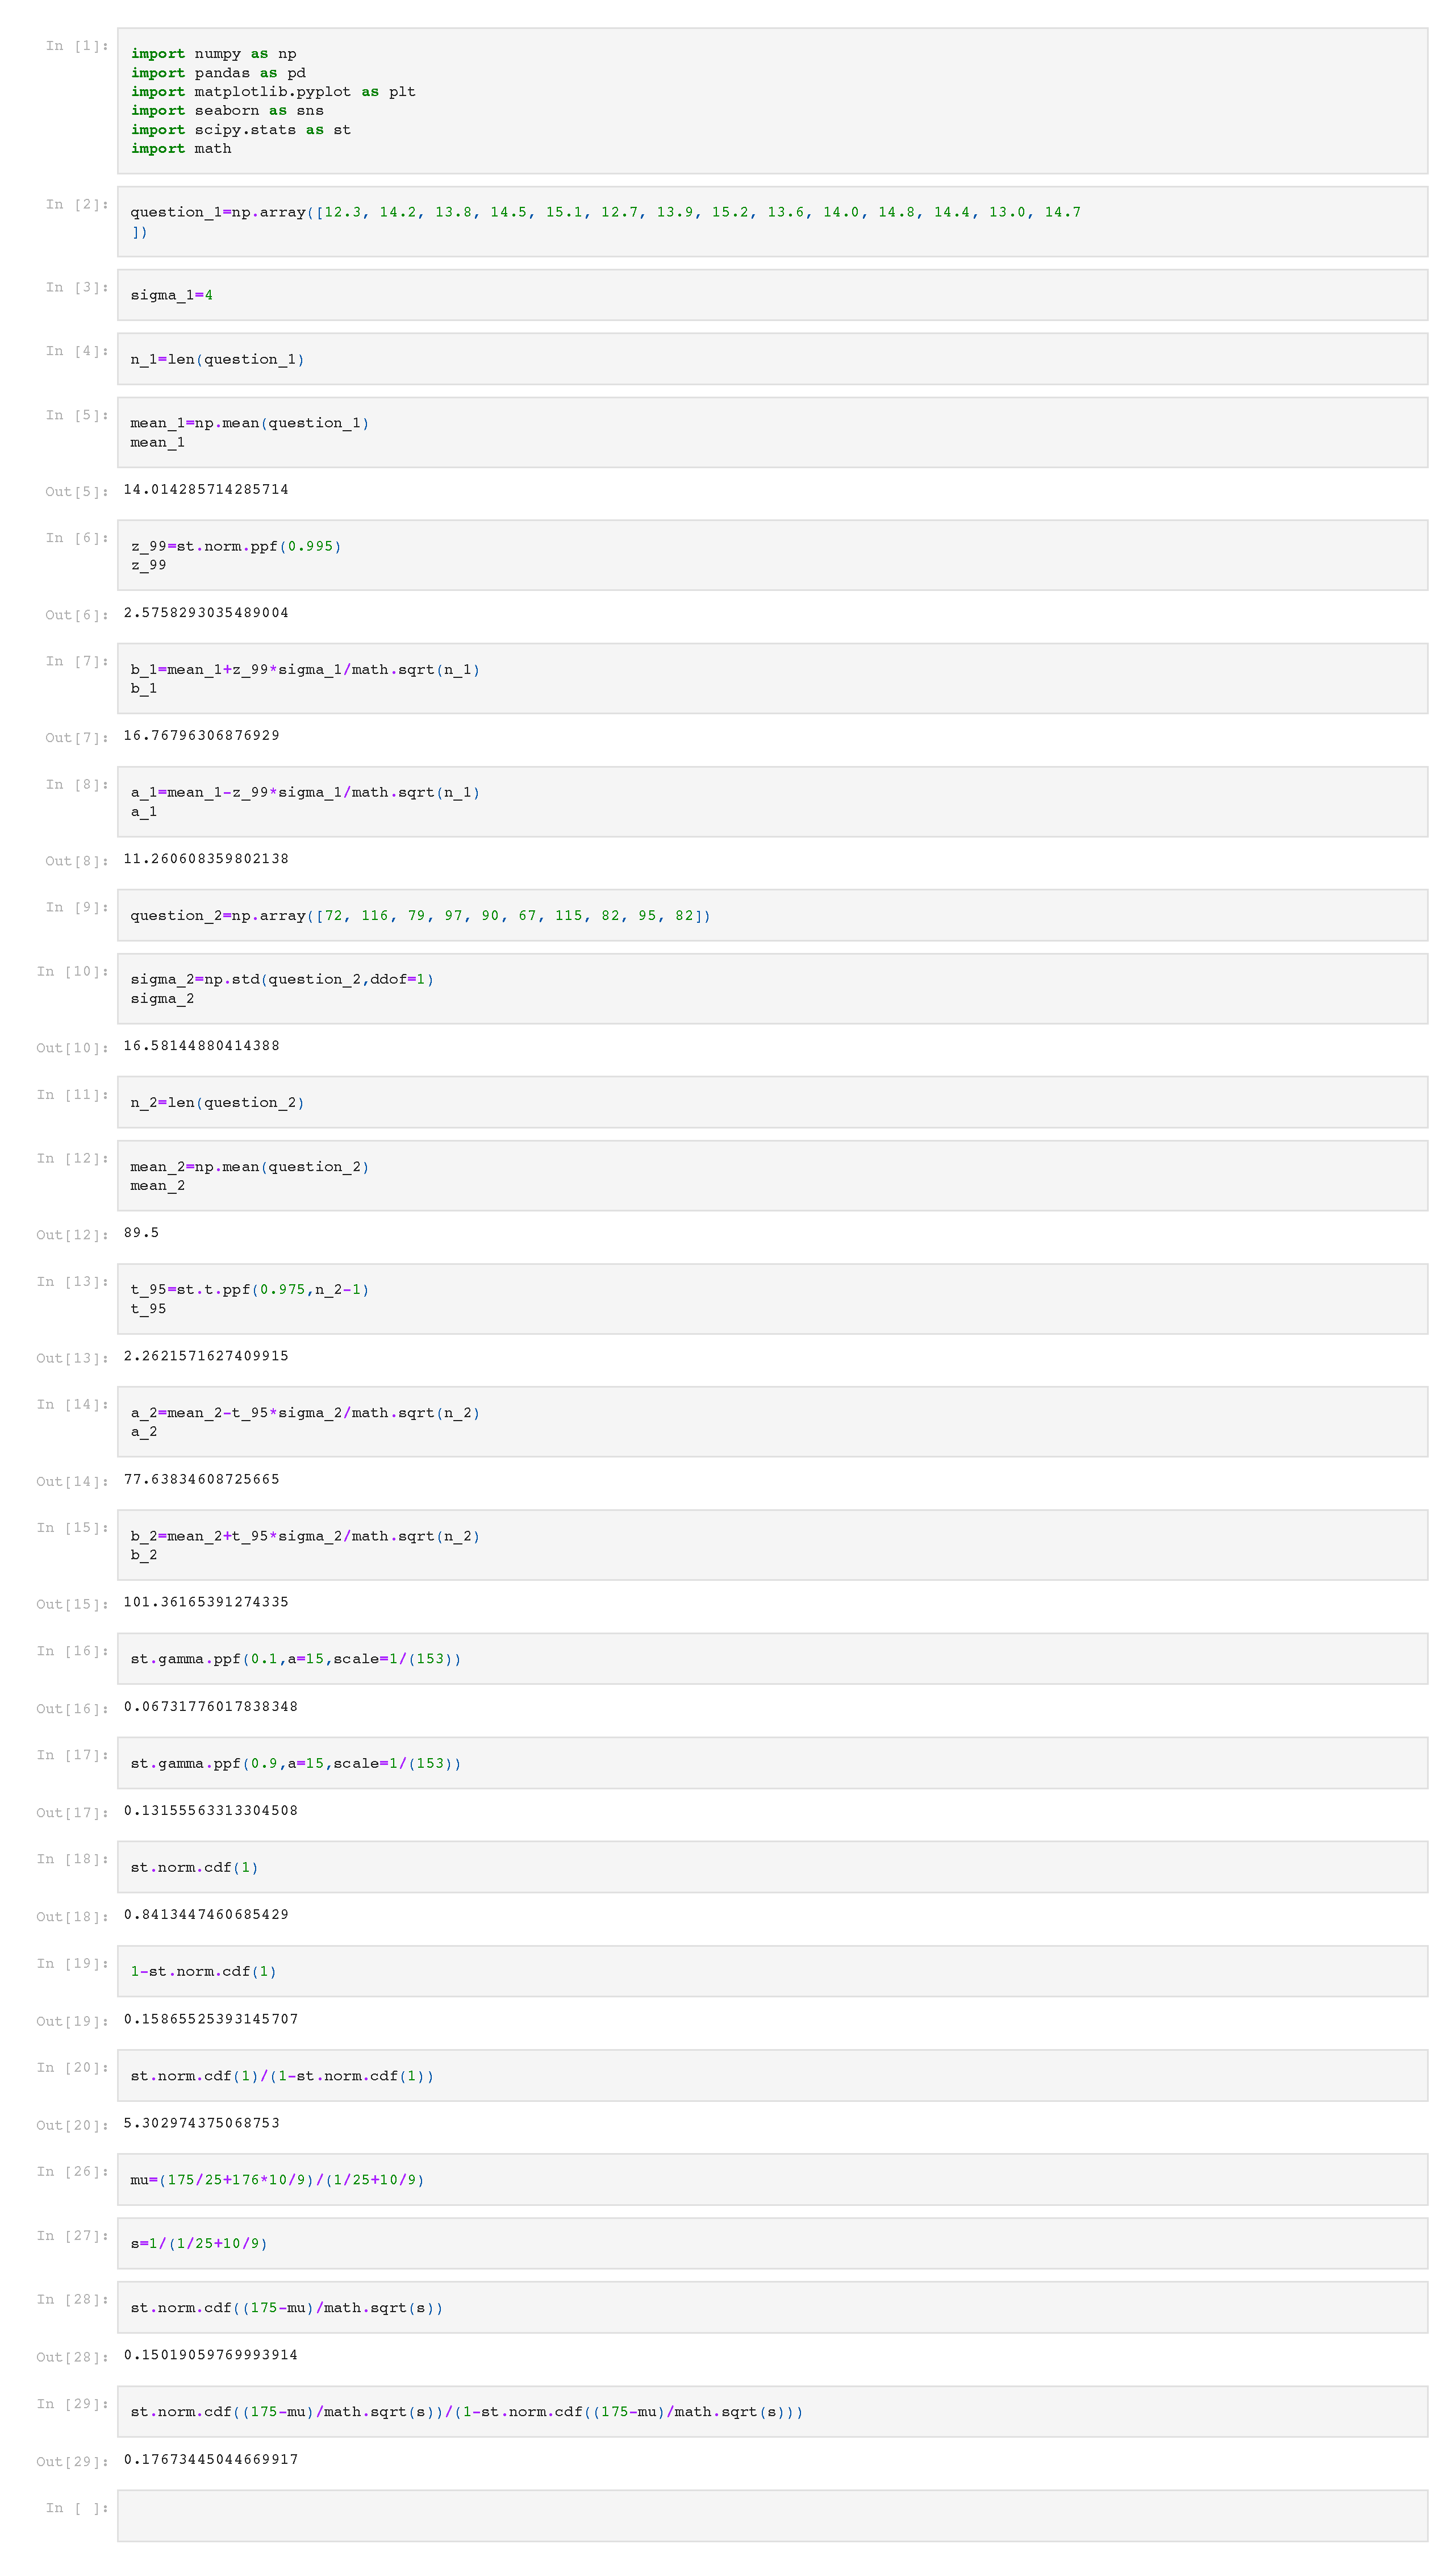
\includegraphics[scale=0.3]{Math 170S homework 3.pdf}
\end{figure}
\end{document}